\chapter{Reinforcement Learning Model}
\label{chap:RLModel}
\section{Introduction}
In the last session we analyzed the task-related activity patterns of principal assembly-pair types.\\Significant task related activity was tested with Friedman test in stimulus presentation (CS+/-) interval, stimulus continued\footnote{The window right before the reward delivery time, or the expected reward time in False Alarm trials, or the hypothetical reward time in Correct Rejection trials.} (CS+/- cont.) interval, and reward\footnote{Or expected reward in False Alarm trials, or Hypothetical Reward in Correct Rejection trials.}.\\We found a good portion of SPN-DAN pairs becoming active early at stimulus presentation, another important group being active later during the stimulus presentation, and only a small fraction of SPN-DAN pairs active only at the retrieval.\\The described activity pattern makes SPN-DAN pairs good candidates for reward prediction (RP) and reward prediction error (RPE) coding.\\On the other hand we observed that FSN-DAN pairs are early activated by the stimulus on onset and they phasic activate at the reward time.\\While in False Alarm a good portion of FSN-DAN is depressed before and after the expected reward time. Such activity could reflect motivational feelings of the animal during the task, that are partially involved in the reward prediction error definition.\\The analysis of task related responses cannot read the highly dynamic of task, the task was indeed such that the animal had to assign and re-assign a value to the rewarded odor to be able to predict the reward. Only taking in account this dynamic we can understand whether and how SPN-DAN and FSN-DAN pairs compute reward prediction error, and if different cell-assembly types specialize in different aspects of the complex task-related coding.\\To take all this into account, we used the reinforcement learning technique \cite{SuttonBarto}. $"$Reinforcement learning$"$ is an area in machine learning, in which an agent tries to learn the best action to take, depending on the circumstances in which this action will be performed, this approach can incorporate any changes in the environment of the decision making process. In psychology, from where the idea of this machinery derives, the concept is known as “learning by reinforcement”: the agent receives a reward or punishment, depending on the decision made, through the experience he is able to associate the actions that generate the greatest reward for each situation that the environment presents, and to avoid unrewarded actions or actions that generate punishment.\\
Machine learning uses the same idea: the machine observes a state and, based on this, chooses an action to take and receives the reward associated with that specific action in that state, thus obtaining the information of this specific combination. The process is repeated until the machine is able to choose the best action to take for each of the possible scenarios to be observed in the future.\\In the contingencies of the experiment conducted in our lab, two odor were presented and only one was associated with a reward with a probability of 0.9. Each time one odor was presented the mouse chose to take the action (lick or not lick) that maximized the reward and minimized his effort. the task was learnt when the animal was able to lick for the rewarded odor and not lick when the unrewarded odor was presented.\\To model this learning process we set up a Rescorla Wagner model with Pearce Hall update mechanism (\cite{Li}, \cite{Costa}, \cite{Koppe}).\\

%%
%We use here Reinforcement Learning/Forgetting models (\cite{SuttonBarto}) with Q-learning values (\cite{Dayan1}) to fit mice behaviour in go-no go odor discrimination task; we regress afterwards neuronal activity with model values.
\section{Model}
%%%%%{\color{blue}Start writing equation of reinforcement learning}
%%%%%First Option I tried, Georgia's option {\color{red}cite Georgia's paper}
%%%%%We set up four RL models and we chose the one that better fitted the behaviour for the regression analysis.
Reinforcement learning model are usually set up as follows:
\begin{itemize}
    \item At each trial $t$ of the experiment, a state $s$ is observed, this is an input of the model.
    \item After the stimulus presentation, the animal has the chance to take an action, and according to choice made, the reward is delivered. The reward is a vector $r(t)$, each vector component indicates the reward value delivered at the trial $t$, the reward vector is an input of the model.
    \item After the reward delivery, the animal computes the reward prediction error, that is evaluated in the model as the difference between the actual reward and the expected reward.
    \item States values are the expected reward values and they are updated according to the last expected values and the reward prediction error and it is modulated by the learning rate.
    \item The learning rate is often a constant free parameter, however it has been shown that a time dependent variable better describes the learning dynamic (\cite{Funamizu}, \cite{Daw}).
    \item Learned values are then translated into action probabilities via a softmax function, maximized with respect some free parameters.
\end{itemize}

We set up a Q Learning-Forgetting model (Q L-F model) starting from an hybrid Rescorla-Wagner/Pearce-Hall update mechanism (\cite{Koppe}, \cite{Costa}, \cite{Li}) with update of unchosen option (\cite{Katahira}) and the associability related to the chosen and unchosen options, using learning and forgetting parameters ({\color{red} cite Dayan, literature on Q L-F models}).
The model assigns each state $s$ and action $a$, an action value $Q_{s,a}(t)$ where $t$ is the index of the trial. In our specific case we have two states, corresponding to the two odors presented and two possible actions, i.e., to lick or not to lick. 
Based on the set of action values the model transforms the The action value for the chosen option is updated by
\begin{equation}
Q_{s,a}(t+1)  = Q_{s,a}(t)+k_L\cdot\alpha_L(t)\cdot\delta(t), \hspace{0.3cm} with \hspace{0.3cm}\delta(t)=r(t)-Q_{s,a}(t)
\label{eq:Qlearning}
\end{equation}
where $\delta$ is the prediction error, i.e., the difference between the reward $r(t)$ and the expected reward value $Q_{s,a}(t)$ for an action $a$ given a state $s$, $k_L$ is the learning parameter and $\alpha_L(t)$ is the Pearce-Hall associability for the chosen option, is a trial-dependent rate component which adjusts in accordance with the average accuracy of recent predictions, evolving by
\begin{equation}
   \alpha_L(t)=(1-\eta)\cdot\alpha_L(t-1)+\eta\cdot\abs{\delta(t)},\hspace{0.3cm} \eta\in[0,1]
    \label{eq:Alphalearning}
\end{equation}
Note that the $n$'s associability depends on absolute prediction errors from past trials, but not the current one ensuring that $\delta(t)$ was not double counted in the value update.\\The associability term in eq. \ref{eq:Alphalearning} measures the attention that the animal has to put to the cue, in other terms it is nothing but the uncertainty of the animal to get the reward. 
For the unchosen option $a'\neq a$ the action value is updated by
\begin{equation}
    Q_{s,a'}(t+1) = Q_{s,a'}(t)-k_F\cdot\alpha_F(t)\cdot Q_{s,a'}(t)
    \label{eq:Qforgetting}
\end{equation}
where $k_F$ is the forgetting rate (\cite{ItoDoya}) and the associability for the unchosen option is time-dependent and evolves as follows
\begin{equation}
    \alpha_F(t)=(1-\eta)\cdot\alpha_F(t-1)+\eta\cdot Q_{s,a'}(t-1), \hspace{0.3cm}
    \eta\in[0,1]
    \label{eq:Alphaforgetting}
\end{equation}
Note that using $k_F = 0$ the model is reduced to the basic Rescorla Wagner/Pearce Hall model. We applied to our data four different version of the model, the one shown here as presentation is the one that better fit the behavioural data. The other three versions are:
\begin{description}
    \item[i.] \textbf{Rescorla-Wagner.} The presented model is reducible to an hybrid Rescorla Wagner/Pearce Hall update mechanism when we use a learning parameter $k$, and no forgetting parameter, i.e. $k_F = 0$.
    Then, if $a$ represents the chosen option and $a'\neq a$ the unchosen option, the action values evolve as follows\\
    $\begin{array}{lcl}
    Q_{s,a}(t+1)&=& Q_{s,a}(t)+k\cdot\alpha_L(t)\cdot\delta(t), \hspace{0.3cm} with \hspace{0.3cm}\delta(t)=r(t)-q_{s,a}(t)\\
    Q_{s,a'}(t+1)&=&Q_{s,a'}(t)\\
    \end{array}$
    \item[ii.] \textbf{Rescorla-Wagner with two learning rate modulations.} Let $a(t) \in \{1,0\}$ denote the option was chosen at trial $t$, where $1$ stands for "to lick" and $0$ stands for "not to lick". We introduce then two learning parameters $k_{1}$ and $k_{0}$ respectively for the choice $a=1$ and $a=0$ to be estimated by the model, while $k_F$ is fixed to zero.
    Then when the choice $a=1$ is realized, the action values evolves by\\
   $\begin{array}{lcl}
       Q_{s,1}(t+1)&=&Q_{s,1}(t)+k_1\cdot\alpha(t)\cdot\delta(t)\\
         Q_{s,0}(t+1)&=&Q_{s,0}(t)\\ 
    \end{array}$\\
    while if the choice $a=0$ is realized we have\\
    $\begin{array}{lcl}
       Q_{s,0}(t+1)&=&Q_{s,0}(t)+k_0\cdot\alpha(t)\cdot\delta(t)\\
         Q_{s,1}(t+1)&=&Q_{s,1}(t)\\ 
    \end{array}$
    \item[iii.] \textbf{Rescorla-Wagner with two $\eta$ parameters.} We use a learning model, without forgetting parameters, and we introduce two $\eta$ parameters $\eta_1$ and $\eta_0$ for the choice $1$ and $0$ respectively, to be estimated by model. The associability $\alpha_L$ evolves as follow:\\
   $\begin{array}{lcll}
    \alpha_{L}(t) & = & (1-\eta_1)\cdot\alpha_{L}(t-1)+\eta_1\cdot\abs{\delta(t)} & \mbox{if\,\,}  a=1,\\
    \alpha_{L}(t) & = & (1-\eta_0)\cdot\alpha_{L}(t-1)+\eta_0\cdot\abs{\delta(t)} & \mbox{if\,\,}  a=0.\\
    \end{array}$\\
    and action values for the chosen option evolving consequently as in the equation \ref{eq:Qlearning}.
\end{description}
\section{Goodness of Fit}
\label{sec:Behavior}
The hybrid Rescorla-Wagner model (i.) has fewer parameters with respect to the three adapted Rescorla-Wagner versions proposed (ii.,iii., L-F model), and all the three versions can be transformed to the hybrid Rescorla-Wagner by imposing constraints on the former's parameters. Thus using Likelihood Ratio tests for nested models we could test for each alternative model proposed whether it was better than the hybrid Rescorla-Wagner.({\color{red}insert reference})Likelihood ratio test (LRT) is formalize as the ratio of the likelihood functions of the models to compare: 
\begin{equation}
LRT = -2 \log (\frac{\mathcal{L}_s(\hat{\theta})}{\mathcal{L}_g(\hat{\theta})})
\label{eq:LRT}
\end{equation}
where $\hat{\theta}$ are the parameters values that maximize the likelihood function.
The simpler model (s) has fewer parameters than the general model (g), the latter can be reduced to the simpler model after imposing some constraint (null hypothesis).\\
LRT compares the fit of two models and has an asymptotic $\chi^2$ distribution. The null hypothesis is that the smaller model is the $"$best$"$ model.  The null hypothesis is rejected when the test statistic is large. In other words, if the null hypothesis is rejected, then the larger model is a significant improvement over the smaller one.\\
In this way in each test we tested whether the addition of one parameter to the pure Rescorla-Wagner model was needed and brought an improvement. The tests were conducted separately for each animal.\\In the comparison between the Rescorla-Wagner and the Learning-Forgetting, the second model reveals to be the $"$best$"$ model for each animal.{\color{red}show pvalues in a tables}
A further test was needed to understand whether the Learning-Forgetting was the best model among the three adapted version of the hybrid Rescorla-Wagner. In this case the best model was evaluated using the Bayesian Information Criterion (BIC), that is is a criterion for model selection among a finite set of models where the model with the lowest BIC is preferred. BIC is formally defined as (\cite{Schwarz})
\begin{equation}
    BIC=k\log(n)-2\log(\hat{\mathcal{L}})
\end{equation}
where:
${\hat{\mathcal{L}}}$ is the maximized value of the likelihood function of the model, $n$ is the sample size, $k$ is the number of parameters estimated by the model.
Following Raftery’s approach, we considered that a difference of BIC lower than 2 between two models is barely worth mentioning, a difference between 2 and 5 is positive, a difference between 5 and 10 is strong, and a difference larger than 10 is very strong (\cite{Raftery}).\\
From the Bayesian Information Criterion (BIC) the L-F model resulted to be the best model fig.(\ref{fig:BIC}), confirming the evidences of the action values plots in fig.(\ref{fig:PerfRL}).
{\color{red}Missing: BIC PLOT. Proper BIC discussion!!! }
\begin{figure}
    \centering
    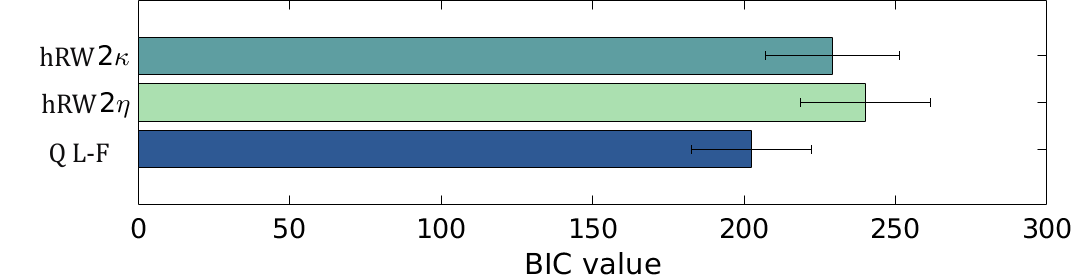
\includegraphics[scale=0.5]{figures/BIC_Value.png}
    
    \vspace{1cm}
    
    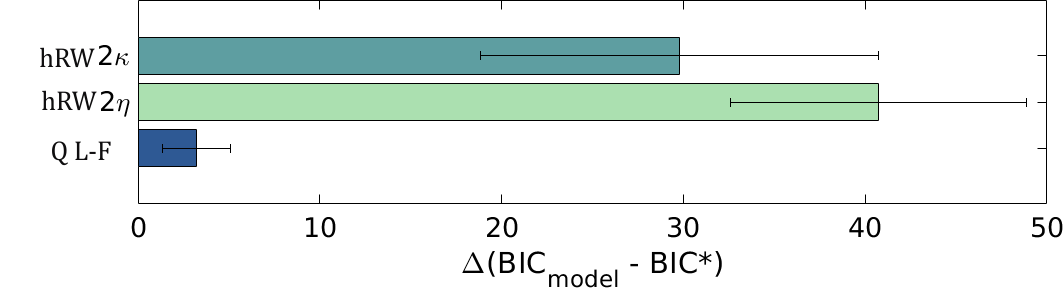
\includegraphics[scale=0.5]{figures/DeltaBIC.png}
    \caption{On top BIC Information Criterion for the three models proposed as alternative of the hybrid Rescorla-Wagner. The BIC was computed separately for each animal, and we report the mean and the standard error. The best model is the model with the lower BIC, indicated as BIC*. The L-F model revealed to be the best model for the more than 80$\%$ of the animals. The $2\eta$ model was never the best model and the $2\kappa$ model was the best model for less the 20$\%$ of the animals, it is worth to notice that also when the L-F model was not the best model, the difference between its BIC and the BIC* rarely passed the value 5. On bottom the difference between the BIC of each model (BIC$_{model}$) and BIC*, this difference was computed separately for each animal and we report the mean and the standard error.}
    \label{fig:BIC}
\end{figure}
\begin{figure}
\centering
    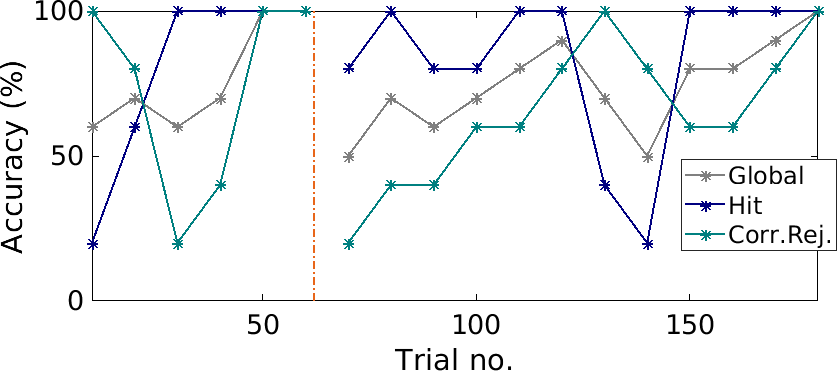
\includegraphics[scale=0.42]{figures/PerfEndrevAn1.png}
    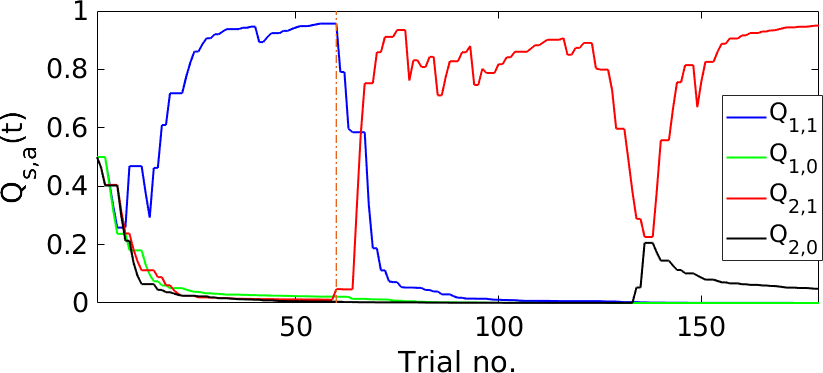
\includegraphics[scale=0.42]{figures/QValuesEndrevAn1.png}
    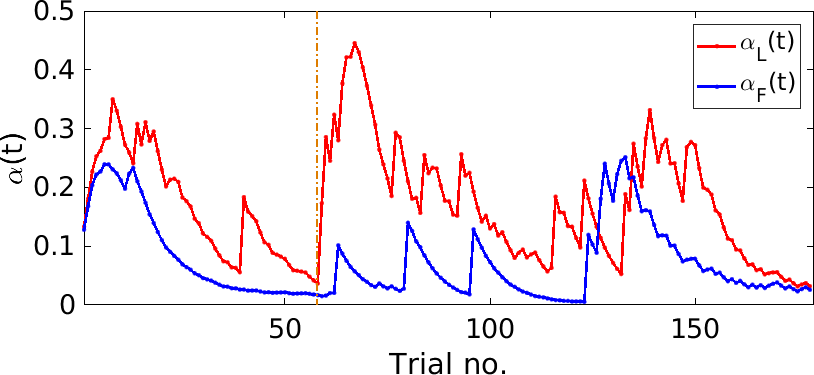
\includegraphics[scale=0.42]{figures/AlphaEndrevAn1.png}
    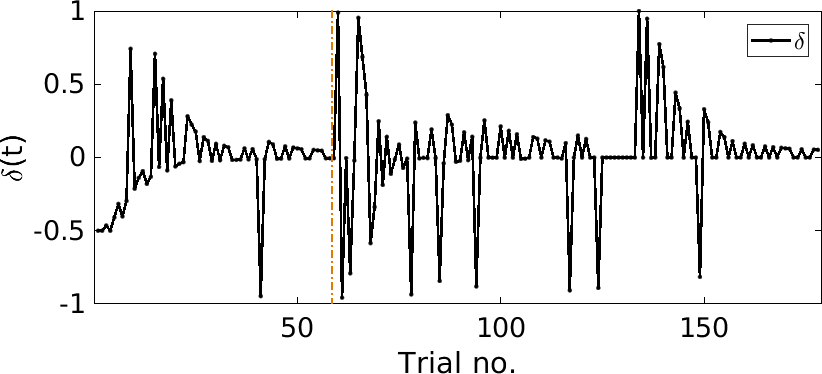
\includegraphics[scale=0.42]{figures/DeltaEndrevAn1.png}
    \caption{In figure one example of animal performance and RL model action values.
    Odor 1 was rewarded only in the original phase, while Odor 2 was rewarded only in the reversal phase. Top: Performance in all trials, in hit trials and correct rejection trials. Bottom: RL model action values for the action lick, when odor 1/odor 2 occurs (blue/red) and the action no lick when odor 1/odor 2 is presented (green/black).}
    \label{fig:PerfRL}
\end{figure}
In figure one example of animal performance and RL-models action values. When the odor is rewarded the expectancy of reward related to the lick action reproduce the hit performance as one could intuitively predict, while, for non rewarded odor, the reward expectation associated to the no-lick action decrease as the correct rejection performance increase. Action values associated to lick for non rewarded odor and non-lick for rewarded odor give us an estimation of $"$false alarm$"$ and $"$miss trials$"$, namely respectively trials in which the odor was not rewarded and the mouse went for the reward, or in which the odor was rewarded and the mouse sat quiet. That happened especially as the experiment or the new phase began for the first 5-10 trials of the phase.\\
%To see whether the neural activity is correlated with the behaviour, we regress the neuronal activity and the assembly activity with the Q L-F model action values $Qs$, error prediction $\delta$, and associability $\alpha$ and behavioural measures. 
\section{Uncertainty and prediction error signal in pair-types}
\label{sec:CorrRL}
We assume VS-VTA interactions being able to predict the reward and compute prediction error. We used a reinforcement learning model to parameterize the learning functions, if the assembly-pairs code for some aspects of the learning they correlate with some reinforcement learning functions.\\
In \hyperref[sec:TaskResp]{~Section \ref*{sec:TaskResp}} we hinted which kind of trial variability in assembly activity we expect when the assembly predicts the reward and computes prediction error, doing a parallelism with the dopamine neurons response in case of probabilistic reward \cite{Fiorillo}.\\
If the assembly-pairs activity codes for the reward prediction we expect intense activity in the CS window during the stable phase, when the animal is able to predict the reward, this case in the probabilistic reward comparison is similar to the case in which the probability to get the reward is equal to 1 or high (see fig. \ref{fig:RewPred} top); whereas during the unstable phase we expect few activation in CS window because the animal is uncertain to get the reward, this case sis comparable with the case of reward probability equal to 0.25 or below (see fig. \ref{fig:RewPred} bottom). In other words we expect the assembly-pair activity in CS window to anti-correlate with the uncertainty $\alpha_L(t)$, indeed the uncertainty is high at the beginning of the task and goes down at the end of the original phase, to raise up again at the beginning of the reversal phase. 
\begin{figure}
    \centering
    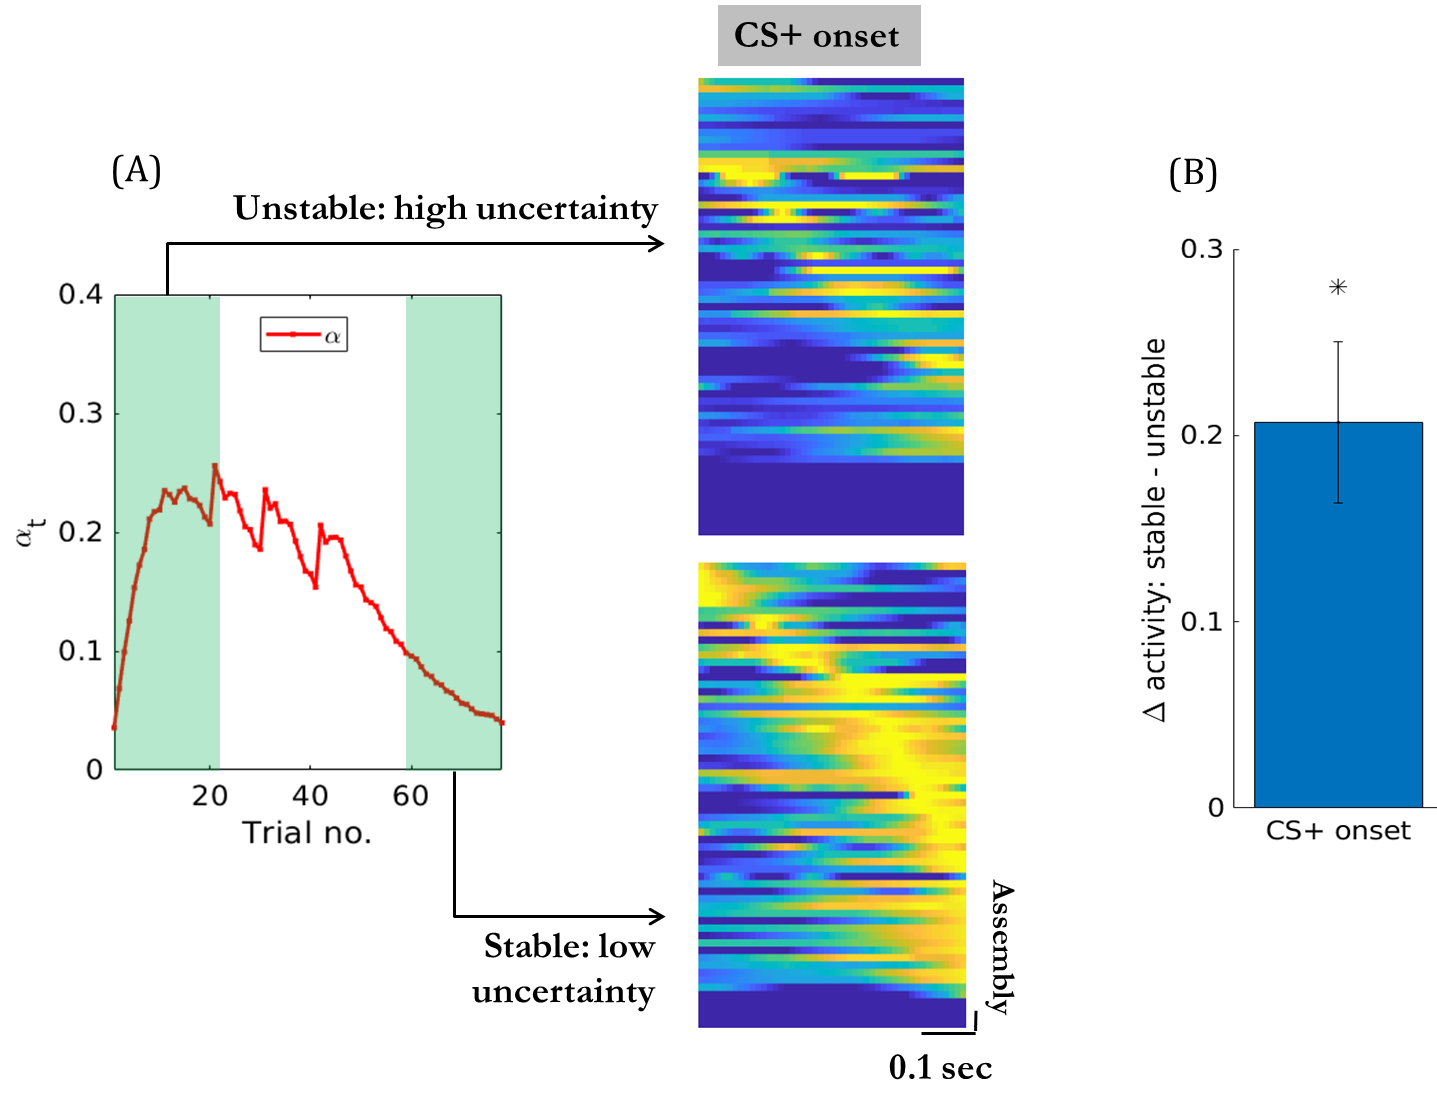
\includegraphics[scale=0.6]{figures/PreRegress.png}
    \caption{(A) Comparison between the uncertainty $\alpha(t)$ and the SPN-DAN assembly pairs activity in the stable and unstable phase. For this example only trials in which the rewarded odor was presented are shown. The analysis was restricted to the CS window, because the prediction of the reward happens immediately after the stimulus onset. If assembly pairs code for reward prediction, in the unstable phase characterized by high uncertainty to get the reward the assembly-pairs activity in CS window is low, whereas in the stable phase characterized by low uncertainty the assembly-pairs activity is high. The difference between the assembly-pairs activity in stable and unstable phase is significantly different to zero (B).}
    \label{fig:StableUnstableAlphaCS}
\end{figure}In fig. \ref{fig:StableUnstableAlphaCS} we show an intuitive way to use the task variability in order to see the correlations with model functions. We divided the task in two phases: a first phase constituted by first trials in which we think the animal is learning the task and is uncertain about the reward outcome, we call this phase the unstable phase; a second phase is on the other hand constituted by last trials of the task in which the animal has learnt the task rule and it is more certain about the reward outcome when a rewarded or unrewarded odor is presented.\\We compare the assembly-pairs activity in unstable and stable phase. The difference between the two phases is significantly different from zero only for SPN-DAN pairs.\\This found highlights a possible specificity of assembly-pairs types coding, that will be proved in the next sessions.\\
With similar arguments we can assume that, if the assembly-pairs compute reward prediction error their activity should correlate with the prediction error $\delta(t)$ in the US window. At the beginning of the task, when the prediction error is high we expect in US window high assembly-pairs response in conformity with the high surprise of the animal to get the reward, while when the task is learnt the surprise to get the reward and the prediction error are smaller and we expect less activity.\\
In order to prove that there is a specific VS-VTA interaction path involved in the reward prediction coding and prediction error computing, we regress the assembly-pair activity with the uncertainty $\alpha (t)$ and prediction error $\delta (t)$ functions of the reinforcement learning model (Q learning-forgetting model).
%We carried out a multiple regression analysis of neuronal and assembly's activity by the four action values of the Q F-L model, $\delta(t)$, $\alpha_L(t)$ and $\alpha_F(t)$. To further test whether the neuronal and assembly activities were correlated with the parameters of subsequent lick movements, or the odor identity, we analyzed the residual components, $\epsilon(t)$, using lick related variables and the odor identity, namely, the mouse's action choice $a(t)$, the lick frequency within the lick-window $l_{in}(t)$, the lick frequency outside the lick-window, before the opening,$l_{out}(t)$ and the odor identity $o(t)$.
%Thus we model the neuronal or assembly activity $y(t)$ during the post-stimulus, pre-reward and post-reward periods in the $t-th$ trial as follows:\\
%\begin{equation}
%\begin{cases}
%y(t)=b_0+\sum\limits_{l}^{L} b_l\cdot M_l+\epsilon(t)\\
%\epsilon(t)=\sum\limits_i^I c_i\cdot N_i
%\end{cases}
%\label{eq:MultiLinRe}
%\end{equation}
%where $y$ are the observations, the neuronal{\color{blue}/assembly's} activity in this case, $M$ is the ($T\times L$) regressor's Matrix of the Q L-F model part, where $T$ is the number of trials and $L$ the number of regressors. $M$ has as columns
%the regressors of the model's part, namely, the vectors $Q_{1,1}$, $Q_{1,0}$, $Q_{2,1}$, $Q_{2,0}$, $\delta$, $\alpha_L$, $\alpha_F$; the set of values $b_m$ are regressor parameters or weights related to the model's regressors. $N$ is the ($T\times I$) regressor matrix of the residual part, where $I$ is the number of regressors of the residual part. N has as columns the regressors $a$, $l_{in}$, $l_{out}$ and $o$, while $c_i$ are the weights of the residual part.
%Linear regression models assume response variables to be normally distributed. Neuronal responses are Poisson distributed (although the normal distribution is in this case a good approximation), {\color{blue} and assemblies show Gamma distribution,} thus considering our data distributions, we built a generalized linear model (GLM), with GLM is possible to generalize the simple linear regression by allowing for response variables that have arbitrary distributions and for an arbitrary function of response variables, the link function, to vary linearly with the predicted values, rather than assuming that the response itself must vary linearly. The mean $\mu$ of distributions depends on the independent variables, or the regressors, $X$, as follows:
%\begin{equation}
%E(Y)=\mu=g^{-1}(X\cdot \beta)
%\label{eq:GLM}
%\end{equation}
%where $g$ is the link function. There is always a well-defined canonical link function which is derived from the exponential of the response's density function. For Poisson observation the canonical link function is the logarithmic. Thus the neuronal activities mean can be expressed by the following:
%\begin{equation}
%\begin{cases}
%\log(\mu)=b_0+\sum\limits_l^L b_l\cdot %M_l+\epsilon(t)\\
%\epsilon(t)=\sum\limits_i^I c_i\cdot N_i 
%\end{cases}
%\label{eq:PoisLinRe}
%\end{equation}

%%%%%%However, in some cases it makes sense to try to match the domain of the link function to the range of the distribution function's mean, or use a non-canonical link function for algorithmic purposes, for example Bayesian probit regression. 
\section{Regression}
\label{sec:Regression}
In the previous sessions we presented the Q learning-forgetting model to parameterize the learning functions. Our main questions are if assembly-pairs predict the reward and compute prediction errors and if different assembly types have different coding features. On this purpose we focus on the uncertainty $\alpha(t)$ and the prediction error $\delta(t)$.
\begin{figure}
    \centering
    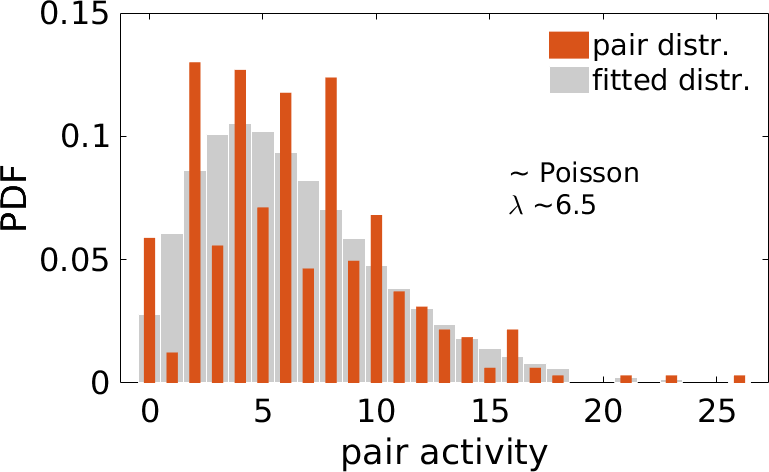
\includegraphics[scale=0.33]{figures/Rev2An2As1_rew.png}
    \hspace{1cm}
    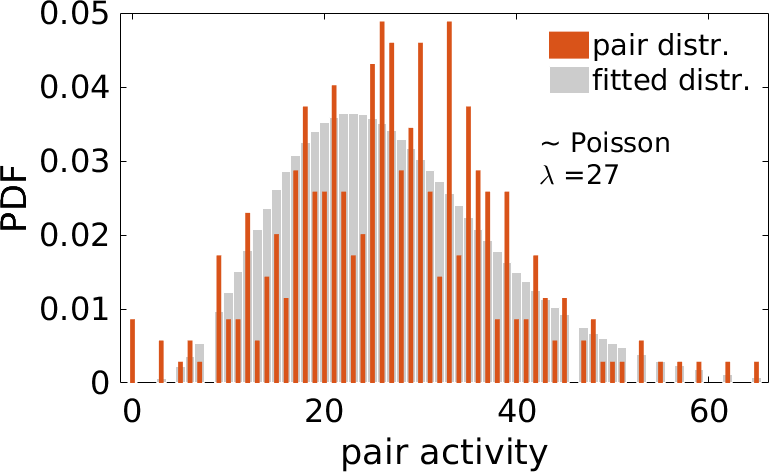
\includegraphics[scale=0.33]{figures/Rev2An2As2.png}
    
    \vspace{1cm}
    
    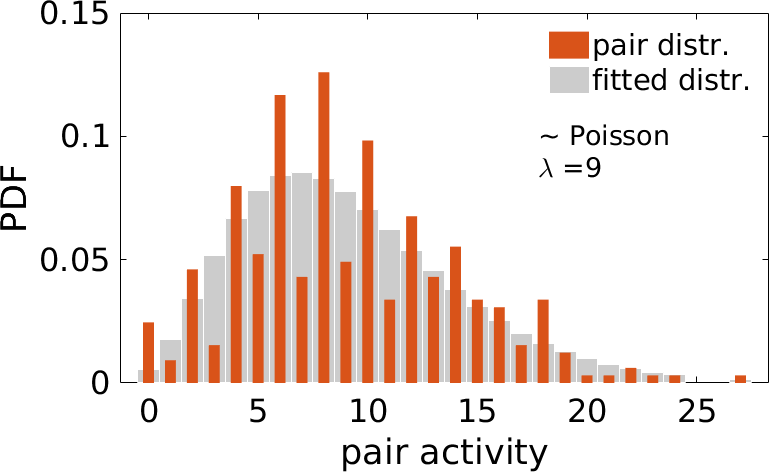
\includegraphics[scale=0.33]{figures/Rev2An2As1.png}
    \hspace{1cm}
    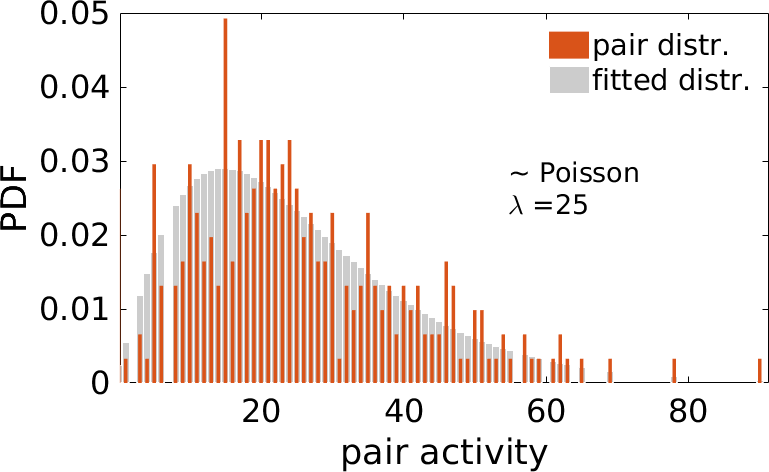
\includegraphics[scale=0.33]{figures/Firstrev1An4As5.png}
    \caption{Some example of pair activity distributions in CS and US window. Assembly-pair distribution can be approximated with Poisson's distribution. To regress out the assembly-pair activity with $\alpha(t)$ and $\delta(t)$ we use a Poisson linear model which is tailored for Poisson distributed observations.}
    \label{fig:DistributionEx}\end{figure}
\section{Conclusion}
%From the regression analysis, as one could predict, VS units emerged to be correlated with the $Q$ values, in particular FSI units show this correlation very clear.


%\begin{figure}
 %   \centering
 %   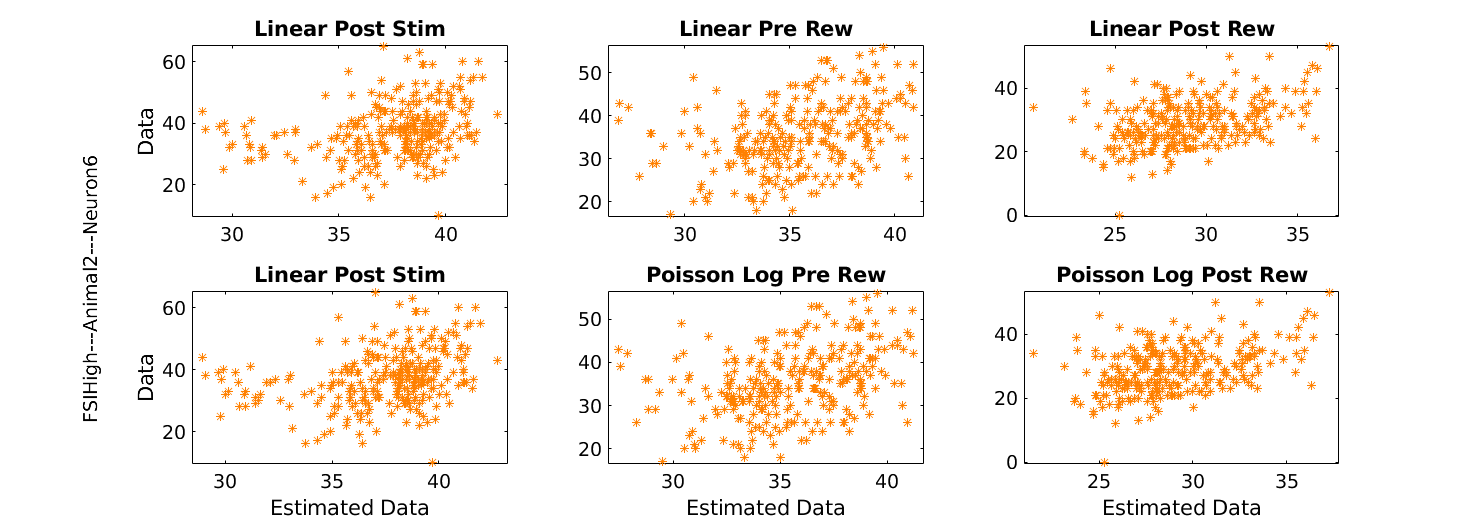
\includegraphics[scale=0.3]{figures/y_yhatAnimal2neu6_FSI.png}
 %   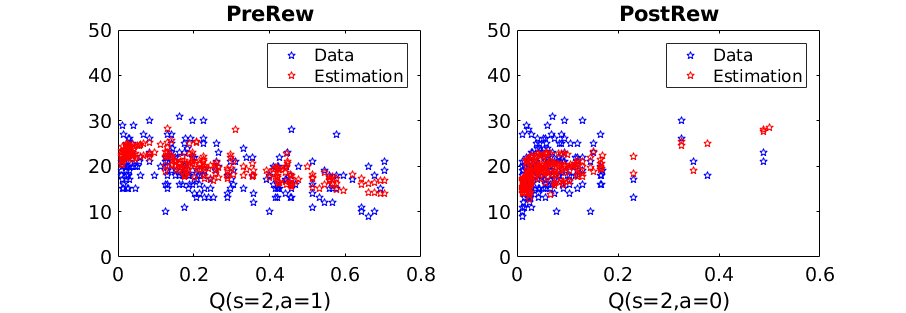
\includegraphics[scale=0.3]{figures/CorrelationExAn1neu6_RightAx.png}
  %  \caption{Caption}
 %   \label{fig:my_label}
%\end{figure}